\section{Asymptotics of the exterior parametrix}
By using the summation formula derived in LV12 the existence and values of the
asymptotic components of the specific operator we're looking at can be
calculated directly. From Lemma bla we know, that we only have to consider $j\in
\{0, 1, 2\}$ since the requested asymptotic coefficient is of order $-5$.

\subsection{Preliminaries}
In (%größtenteils)
accordance with LV12 we denote
\begin{align*}
    % TODO Anständig einführen im Setting, Unterschiede zum LV12-paper ausweisen
    % TODO Explizit darauf hinweisen, dass alle gewöhnlichen Funktionen als
    %      Multiplikationsoperator zu verstehen sind.
    \mu &:= \sqrt{\lambda^2 V(0) + z^2} \\
  % TODO: \lambda(0) = W(0), da \tilde V(x) = V(x) - V(0) = 0 für x = 0
    \lambda(x) &:= \lambda^2 \tilde V(x) + W(x) \\
       k_{R_-} &:= \Eto{-\mu\Abs{x-y}} \\
    k_{R_+} &:= -C(\mu,\theta)\Eto{-\mu(x+y)} \\
    R_\theta &:= \tfrac1{2\mu} (R_- + R_+) \\
    R_{(\sigma_1,\sigma_2,\ldots,\sigma_n)} &:= 
    \left(\tfrac1{2\mu}\right)^n R_{\sigma_1} \lambda(V,W) R_{\sigma_2} \dots
    \lambda(V,W) R_{\sigma_n} \\
    R^{(j)} &:= (-1)^j \psi \left( [R_\theta \lambda(V,W)]^j R_\theta -
    [R_-\lambda(V,W)]^j R_-\right) \phi \\
            &= (-1)^j
                \sum_{
                        \substack{
                          \sigma\in\{+,-\}^{j+1} \\
                         \sigma\neq(-,\ldots,-)
                         }
                        }
                     \psi R_\sigma
                \phi
\end{align*}

We also set
\begin{align}
    \Lambda(x) := \Integ[x]{0}{t}{\lambda(t)}\quad\text{and}\quad
    \mathrm M(x) := \Integ[x]{0}{t}{\Lambda(t)}.
\end{align}

We will need both of the following Lemmas for the calculation. The first one is
a classical result of asymptotic analysis and is the base of all further results
on the asymptotics of exponential integrals.
\begin{Lemma}[Watson]
  Let $\phi\colon [0,1] \to \mathbb{C}, \phi(t) = t^\sigma g(t)$ such that $g$ is
analytic in some neighbourhood of $t=0$, $\sigma > -1$, $\beta > 0$, and
\begin{equation*}
  \exists C, b > 0\, \forall t > 0\colon \Abs{\phi(t)} < C \Eto{bt}.
\end{equation*}
Then the exponential integral
\begin{align*}
  F(x) := \Integ[T]{0}{t}{\Eto{-\beta\,xt}\phi(t)}.
\end{align*}
is finite for all $x \geq 0$ and has the asymptotic expansion in terms of the
gamma function $\Gamma$ (cf.\ \cref{app:gamma})
\begin{equation*}
  F(x)\SimAs{x\to\infty}\sum_{n=0}^{\infty}
  \frac{g^{(n)}(0)}{(\beta x)^{n+\sigma+1}} \frac{\Gamma(n+\sigma+1)}{n!}
\end{equation*}

  \begin{proof}
    Since the proof is a bit lengthy and not needed to understand the following
    it can be found in Appendix~\ref{sec:proof-watson}.
  \end{proof}
%    \begin{Remark}
%        We actually don't need analyticity but only the existence of as many
%        derivatives as degrees we want and additionally a finiteness condition
%        on .
%    \end{Remark}
\end{Lemma}

The second Lemma is a quite general formula for nested integrals, in which the
upper limit of the inner integral is the integration variable of the outer one:
\begin{Lemma}
    \label{lem:triangle-integration}
    Let $f,g\colon[0,1]\to\mathbb{R}$ be continuous. Then the following formula
    holds:
    \begin{align*}
        \Integ[1]{0}{x}{g(x)\Integ[1]{x}{y}{f(y)}} =
        \Integ[1]{0}{y}{f(y)\Integ[y]{0}{x}{g(x)}}
    \end{align*}
    \begin{proof}
        Let $F(x) := \Integ[x]{0}{y}{f(y)}$ and $G(y) := \Integ[y]{0}{x}{g(x)}$.
        Then we see using partial integration:
        \begin{align*}
            \Integ[1]{0}{x}{g(x)\Integ[1]{x}{y}{f(y)}} &=
            \Integ[1]{0}{x}{g(x)F(1)} - \Integ[1]{0}{x}{g(x)F(x)} \\
            &= G(1)F(1) - \left(\Bigl.G(y)F(y)\Bigr|_0^1 -
            \Integ[1]{0}{y}{G(y)f(y)}\right) \\
            &= \Integ[1]{0}{y}{G(y)f(y)} =
            \Integ[1]{0}{y}{f(y)\Integ[y]{0}{x}{g(x)}},
        \end{align*}
        which proves the given formula.
    \end{proof}
\end{Lemma}

\begin{Remark}
  This is in fact only Fubini's theorem for the integral of $(x,y)\to g(x)f(y)$
  over a right-angled triangle:
  \begin{center}
    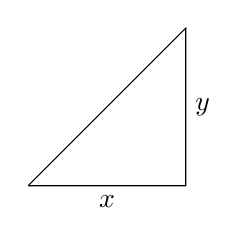
\begin{tikzpicture}
      \draw (0,0)
      -- (2,2)
      -- node[anchor=west] {$y$} (2,0)
      -- node[anchor=north] {$x$} (0,0);
    \end{tikzpicture}
  \end{center}
\end{Remark}

With those given we can explicitly calculate the asymptotics of the
resolvent-trace, which we will do now for $x=0$. The case $x=1$ is identical to
this one if we employ the transformation $x\mapsto 1-x$, which results in a sign
change for odd derivatives of $\lambda(x)$, and of course evaluation at $x=1$
instead of $0$.

\subsection{Calculations}
% TODO
From the above considerations we know that we will have to calculate the
asymptotics of $2^3 - 1 + 2^2 - 1 + 2^1 - 1 = 11$ traces. For symmetry reasons
we can reduce this to 7 integrals. We can do this as we can see in the further
calculation that it suffices to prove the following Lemma:
% TODO: Auswalzen warum Stetigkeit ausreicht.
\begin{Lemma}
  Let $f\colon [0,T)\to\mathbb{R}$ (where $T$ may be $\infty$) be an integrable
  function. Then the exponential parameter integral
  \begin{align*}
    F(x) = \Integ[T]{0}{t}{\Eto{-tx} f(t)}
  \end{align*}
  is continuous in $x$.
  \begin{Proof}
    The statement follows immediately from a classical result of Lebesgue theory
    on the continuity of parameter-dependent integrals (REF: Königsberger 2
    282f). We only need to check, that there is an integrable majorant for all
    $x$, which is simply $f(t)$ in this case, and that the whole integrand is
    continuous in $x$ for fixed $t$ which is obvious.
  \end{Proof}
\end{Lemma}

In the following calculations we define analogous to $R$
\begin{align}
  C_{(\sigma_1,\ldots,\sigma_n)} := \Bigl(-\frac{1}{2\mu}\Bigr)^n
                                    \prod_{
                                      \substack{
                                        1\le i \le n \\
                                        \sigma_i = -
                                    }} -C(\mu,\theta),
\end{align}
which converges to $(-2\mu)^{-n}$ as $\mu\to\infty$, where $k$ is the count
of $(-)$-symbols in $\sigma$, since $C(\mu,\theta)\to -1$ in the non-degenerate
case of $\theta \neq 0$.
% TODO: Fall \theta != 0 genauer erklären (Neumann vs Dirichlet glaub ich)

The calculation of all terms with $\sigma=(+,\ldots,+)$ is straightforward:
\begin{align*}
  \Tr R^{(j)}_{+\ldots+} &=
    C_{+\ldots+}
    \Int{x}{
      \Integ{[0,1]^{j}}{z}{
        \Eto{-\mu((x + z_1) + (z_1 + z_2) + \ldots + (z_j + x))}
        \prod_{i=1}^j \lambda(z_i)
      }
    } \\
    &= C_{+\ldots+}
      \Int{x}{\Eto{-2\mu x}} \left(\Int{z}{\Eto{-2\mu z}\lambda(z)}\right)^j \\
    &= C_{+\ldots+}
      \left(\frac1{2\mu} - \frac{\Eto{-2\mu}}{2\mu}\right)
      \left(\Int{z}{\Eto{-2\mu z}\lambda(z)}\right)^j \\
      &\SimMu (-2\mu)^{-j-2}
      \left(\Wsum{\lambda^{(n)}}\right)^j = (-1)^j (2\mu)^{-2(j+1)}
      \left(\sum_{n=0}^\infty\frac{\lambda^{(n)}(0)}{(2\mu)^n}\right)^j.
\end{align*}
% TODO: Proof of this statement? Im Prinzip geht da auch wieder Stetigkeit ein,
% TODO: Denn wir fassen die Integrale quasi als einzelne Integrale mit
% TODO: unterschiedlichen Parametern (\mu_1, …, \mu_n) auf, auf die nacheinander
% TODO: Watsons Lemma angewandt wird. Für die Partialsummen gilt das
% TODO: offensichtlich, damit sollte das folgen.
The last transformation uses Watson's lemma as well as the fact, that we can
apply it simultaneously to multiple integrals to determine the common
asymptotics, which is ensured by the finiteness of $F(x) =
\Int{x}{\Eto{-tx}f(t)}$. %TODO: Auswalzen, siehe oben

From this calculation we immediately get the first term we were looking for:
\begin{align}
  \label{eqn:tr1}
  \Tr R^{(0)} \SimAs{\mu\to\infty} (2\mu)^{-2}
\end{align}

For the other terms with $j=1$ and $j=2$ we need to employ both Watson's Lemma
and our integration formula. The process is always the same:
\begin{enumerate}
  \item Write down the whole integral with one large exponential
  \item Combine all terms that appear trivially in the exponent (i.e. not in the
    absolute value of a difference) and split of the $\Int{x}{\Eto{-2\mu
    x}\lambda(x)}$-term
  \item For each absolute value of the form $\left|x-y\right|$ in the exponent 
    split the corresponding integral in $x > y$ and $x < y$
  \item The resulting parameter in the integral limits can be coped with using
    the integration formula, which flattens the integral
  \item The integral is now in the form of multiple exponential integrals
    multiplied together, so we apply Watson's lemma on each of them
\end{enumerate}
That way we derive a finite product of infinite sums as the asymptotic
expansion. To get an actual coefficient from that we use combinatorics (we could
of course just combine the sum using the Cauchy product formula, but that will
just result in a much more complicated term).

% j = 1, ++: Oben
% j = 1, +-
In addition to the already calculated $\Tr R^{(1)}_{++}$-term we need to
calculate only this one for $j=1$:
\begin{align*}
  \Tr R^{(1)}_{+-} &= C_{+-} \Int{x}{
      \Int{z}{
        \Eto{-\mu(x+z+\Abs{z-x})}
        \lambda(z)
      }
    } \\
    &= C_{+-} \Int{x}{
      \left(
        \Integ[x]{0}{z}{
          \Eto{-\mu(x+z+x-z)}\lambda(z)
        }
      + \Integ[1]{x}{z}{
          \Eto{-\mu(x+z-x+z)} \lambda(z)
        }
      \right)
    } \\
    &= C_{+-} \left(
      \Int{x}{\Eto{-2\mu x} \Lambda(x)}
      + \Int{x}{\Eto{-2\mu x} \lambda(x)x}
      \right) \\
      % Result:
    &\SimAs{\mu\to\infty} %
      (2\mu)^{-3}\left(
      \Wsum{\Lambda^{(n)}} + \Wsum{n\lambda^{(n-1)}}\right)
      = (2\mu)^{-3} \Wsum[1]{(n+1)\lambda^{(n-1)}},
\end{align*}
since $\Lambda(0) = 0$. We also used the identity $(xf(x))^{(n)} = xf^{(n)}(x) +
nf^{(n-1)}(x)$ (which results in the $n\lambda^{(n-1)}(0)$ term as we evaluate
at $0$) as well as the triangle integration
(Lemma~\ref{lem:triangle-integration}) with $g \equiv 1$.
For the symmetry reasons given above this is also the asymptotics of $\Tr
R^{(1)}_{-+}$, so we have:
\begin{align}
  \label{eqn:tr1}
  \Tr R^{(1)} \SimAs{\mu\to\infty} (-2\mu)^{-4}
  \left(
    \lambda^2\cdot 0 + W(0) + \sum_{n=1}^\infty \frac{
      \lambda^{(n)}(0) + 2(n+1)\lambda^{(n-1)}(0)
    }{(2\mu)^n}
  \right)
\end{align}

% j = 2
The calculations for $j = 2$ are a bit more involved. We start off with the case
$\Tr R^{(2)}_{++-} =  \Tr R^{(2)}_{-++}$:
% -++
\begin{align*}
  \Tr R^{(2)}_{-++} &= C_{-++} \Int{x}{
  \Int{z_1}{
    \Int{z_2}{
      \Eto{-\mu(\Abs{x-z_1} + z_1 + z_2 + z_2 + x)}
      \lambda(z_1)\lambda(z_2)
    }
  }
  } \\
  &= C_{-++} \Int{z_2}{\Eto{-2\mu z_2}\lambda(z_2)}
  \Int{x}{
    \left(
    \Integ[x]{0}{z_1}{
      \Eto{-2\mu x}\lambda(z_1)
    }
    + \Integ[1]{x}{z_1}{
      \Eto{-2\mu z_1}\lambda(z_1)
    }
    \right)
  } \\
  &= C_{-++} \Int{z}{\Eto{-2\mu z}\lambda(z)}
  \Int{x}{\Eto{-2\mu x}(\Lambda(x) + x\lambda(x))} \\
  &\SimMu (2\mu)^{-4} \Wsum{\lambda^{(n)}} \Wsum[1]{(n+1)\lambda^{(n-1)}}.
\end{align*}
Very similar to that we can calculate $\Tr R_{+-+}$:
% +-+
\begin{align*}
  \Tr R_{+-+}^{(2)} &= C_{+-+} \Int{x}{
    \Int{z_1}{
      \Int{z_2}{
        \Eto{-\mu(x+z_1 + \Abs{z_1 - z_2} + z_2 + x)}
        \lambda(z_1)\lambda(z_2)
      }
    }
  } \\
  &= C_{+-+} \Int{x}{\Eto{-2\mu x}}
  \Int{z_1}{
    \left(
    \Integ[1]{z_1}{z_2}{
      \Eto{-2\mu z_2}\lambda(z_1)\lambda(z_2)
    }
    + \Integ[z_1]{0}{z_2}{
      \Eto{-2\mu z_1}\lambda(z_1)\lambda(z_2)
    }
    \right)
  } \\
  &= C_{+-+} \Int{x}{\Eto{-2\mu x}}
    \Int{z}{
      \Eto{-2\mu z}\left(
        \Lambda(z)\lambda(z) + z (\lambda(z))^2
      \right)
    } \\
  % Result
    &\SimMu (2\mu)^{-5} \sum_{n=0}^\infty \frac{(\Lambda\lambda)^{(n)} +
  (z(\lambda(z))^2)^{(n)}(0)}{(2\mu)^{n+1}}
\end{align*}

% --+
Finally we arrive at the two most difficult terms, involving two absolute values
in the exponent, first $\Tr R_{--+}^{(2)}$:
\begin{align*}
  \Tr R_{--+}^{(2)} &= C_{--+} \Int{x}{
    \Int{z_1}{
      \Int{z_2}{
        \Eto{-\mu(\Abs{x-z_1} + \Abs{z_1 - z_2} + z_2 + x)}
        \lambda(z_1)\lambda(z_2)
      }
    }
  } \\
  = C_{--+} \Int{x}{\Bigl( \\
    % (I) x < z_1 < z_2
    &\Integ[1]{x}{z_1}{\Integ[1]{z_1}{z_2}{
        \Eto{-2\mu z_2}\lambda(z_1)\lambda(z_2)
      }
    } \\ &+
    % (III) x < z_1, z_2 < z_1 
    \Integ[1]{x}{z_1}{\Integ[0]{z_1}{z_2}{
        \Eto{-2\mu z_1}\lambda(z_1)\lambda(z_2)
      }
    } \\ &+
    % (IV) x < z_2 < z_1
    \Integ[x]{0}{z_1}{\Integ[z_1]{0}{z_2}{
        \Eto{-2\mu x}\lambda(z_1)\lambda(z_2)
      }
    } \\ &+
    % (II) x > z_1, x > z_2
      \Integ[x]{0}{z_1}{\Integ[1]{z_1}{z_2}{
        \Eto{-2\mu (x + z_2 - z_1)}\lambda(z_1)\lambda(z_2)
      }
    }
    \Bigr)
  }
\end{align*}
After splitting the Integral in those four terms we evaluate them one by one:
\begin{enumerate}[(I)]
  \item Using $\Integ[x]{0}{z}{z\lambda(z)} = x\Lambda(x) - M(x)$ we have:
    \begin{align*}
      \Int{x}{
        \Integ[1]{x}{z_1}{\Integ[1]{z_1}{z_2}{
            \Eto{-2\mu z_2}\lambda(z_1)\lambda(z_2)
          }
        }
      }
      &= \Int{z_1}{z_1 \Integ[1]{z_1}{z_2}{\Eto{-2\mu z_2}\lambda(z_1)\lambda(z_2)}}
      \\
      &= \Int{z_2}{\Eto{-2\mu z_2}\lambda(z_2) \Integ[z_2]{0}{z_1}{z_1\lambda(z_1)}}
      \\
      &\SimMu \Wsum{(x\lambda\Lambda - \lambda M)^{(n)}}
    \end{align*}

  \item
    \begin{align*}
      \Int{x}{
        \Integ[1]{x}{z_1}{
          \Integ[z_1]{0}{z_2}{
            \Eto{-2\mu z_1}{\lambda(z_1)\lambda(z_2)}
          }
        }
      }
      &= \Int{z_1}{z_1 \Eto{-2\mu z_1}\lambda(z_1)\Lambda(z_1)} \\
      &\SimMu \Wsum{(z\lambda\Lambda)^{(n)}}
    \end{align*}

  \item
    \begin{align*}
      \Int{x}{
        \Integ[x]{0}{z_1}{
          \Integ[z_1]{0}{z_2}{
            \Eto{-2\mu x}\lambda(z_1)\lambda(z_2)
          }
        }
      }
      &= \Int{x}{
        \Eto{-2\mu x} \Integ[x]{0}{z_1}{\lambda(z_1)\Lambda(z_1)}
      } \\
      &\SimMu \sum_{n=1}^\infty \frac{(\lambda\Lambda)^{(n-1)}}{(2\mu)^{n+1}}
    \end{align*}

  \item After those pretty straight-forward calculations we are left with a more
    difficult one:
    \begin{align*}
      \Int{x}{
        \Eto{-2\mu x}
        &\Integ[x]{0}{z_1}{
          \Eto{+2\mu z_1} \lambda(z_1)
          \Integ[1]{z_1}{z_2}{
            \Eto{-2\mu z_2} \lambda(z_2)
          }
        }
      } \\
      =&\Int{z_1}{
        \Eto{2\mu z_1}\lambda(z_1)
        \Integ[1]{z_1}{z_2}{
          \Eto{-2\mu z_2}\lambda(z_2)
        }
        \frac{1}{2\mu}\left(\Eto{-2\mu z_1} - \Eto{-2\mu}\right)
      } \\
      =&\ \frac{1}{2\mu}
        \Int{z_1}{
          \lambda(z_1)
          \Integ[1]{z_1}{z_2}{
            \Eto{-2\mu z_2}\lambda(z_2)
          }
        }
        -\frac{1}{4\mu}
        \left(\Int{z}{\Eto{-2\mu z}\lambda(z)}\right)^{2}
        \\
        =&\ \frac{1}{2\mu} \Int{z_2}{\Eto{-2\mu z_2}\lambda(z_2)\Lambda(z_2)}
        -\frac1{4\mu}\left(\Int{z}{\Eto{-2\mu z}\lambda(z)}\right)^{2}
        \\
        &\ \SimMu \sum_{n=1}\frac{(\lambda \Lambda)^{(n-1)}}{(2\mu)^{n+1}}
              -\frac{1}{4\mu}\left(\Wsum{\lambda^{(n)}}\right)^2
    \end{align*}
    % TODO Finalize
\end{enumerate}
which leads us to
\begin{align*}
  \Tr R_{--+}^{(2)}
  &= (2\mu)^{-4} \sum_{n=1}^{\infty}
  \frac{
    (M + 2x\lambda\Lambda)^{(n)}(0)
    + 2(\lambda\Lambda)^{(n-1)}(0)
  }{(2\mu)^n}
\end{align*}

% -+-
\begin{align*}
  \Tr R_{-+-}^{(2)} &= C_{-+-} \Int{x}{
    \Int{z_2}{
      \Int{z_1}{
        \Eto{-\mu(\Abs{x-z_1}+z_1+z_2+\Abs{z_2-x})}\lambda(z_1)\lambda(z_2)
      }
    }
  } \\
  &= C_{-+-} \Int{x}{
    \Eto{-2\mu x}
    \left(
      \Lambda(x)^2 + 2\lambda(x)M(x)
      % TODO: Dritter Term ist noch nicht 
      % gerechnet!
    \right)
  }
\end{align*}

Now that we have calculated all those terms we only need to sum them up and
match coefficients to get the first three terms in the asymptotic expansion of
$\Tr(\Delta_\lambda + z^2)^{-1}$. In particular we have to deal with the fact,
that $\lambda(x) = \lambda^2 V(x) + W(x)$ is of mixed order. Furthermore we note
that, as it was for the interior parametrix, the coefficients of the trace
expansion are again a homogeneous polynomial in $V$, $W$ and their respective
derivatives. Assuming that we can carry on with our method (which is possible
though highly tedious) this will also hold for higher orders, since it will by
construction only produce positive integer powers of $\lambda(x)$ and its
derivatives.
% TODO: PROOF, das ist wichtig (sagt Lesch!)
%       Annahme dazu: Wir können jedes Integral der Art \Tr R_{+-+-+-+…}^{(n)}
%       in eine Form bringen, so dass Watson's Lemma angewandt werden kann.

Summing up the previous results we get the following three terms of the
asymptotic expansion of $\Tr R_\theta$:
\begin{align}
  h_1 &= \frac{1}{4\mu^2} = \frac{1}{4} (\lambda^2 + z^2)^{-1} \\
  h_2 &= \frac{\lambda^2}{(2\mu)^5} V'(0) \\
  h_3 &= \frac{\lambda^4}{(2\mu)^8} \frac12 (V'(0))^{2}
       + \frac{\lambda^2}{(2\mu)^6} \left(V''(0) + 6V'(0)\right)
       + \frac1{(2\mu)^4} W(0).
\end{align}

We have thus proven the following theorem
\begin{MainTheorem}
  The multiparametric trace-expansion of the resolvent of the Sturm-Liouville
  operator
  \begin{align*}
    \Delta_\lambda = -\partial_x^2 + \lambda^2 V(x) + W(x)
  \end{align*}
  up to the third non-vanishing order is given by
  \begin{align*}
    \text{kommt noch}
  \end{align*}
\end{MainTheorem}
